

% Useful macros
\newcommand{\otb}{\textbf{Orfeo ToolBox}\xspace}
\newcommand{\app}{\textbf{OTB Applications}\xspace}
\newcommand{\mont}{\textbf{Monteverdi}\xspace}
\newcommand{\montNew}{\textbf{Monteverdi2}\xspace}
\newcommand{\jpg}{Jpeg2000}\xspace}
\newcommand{\phr}{Pleiades}\xspace}
\newcommand{\mmod}[1]{\emph{#1}\index{#1}\xspace}
\newcommand{\application}[1]{\emph{#1}\index{#1}\xspace}
\newcommand{\ossim}{OSSIM}\xspace}
\newcommand{\sg}{OTB Software Guide}\xspace}
\newcommand{\dox}{Doxygen}\xspace}
\newcommand{\website}{Orfeo ToolBox website}\xspace}
\newcommand{\qgis}{Quantum GIS}\xspace}
\newcommand{\gdal}{GDAL}\xspace}
\newcommand{\osgeow}{OSGeo4W}\xspace}
\newcommand{\download}{OTB download page}\xspace}
\newcommand{\googleearth}{\textbf{Google Earth\copyright}\xspace}

\newtheorem{algo}{Algorithm}
\newtheorem{defin}{Definition}


%
%  Change this to say a4paper instead of letterpaper if you want A4.  These
%  are the latex defaults.
%
\newcommand{\itk@paper}{letterpaper}
\newcommand{\itk@ptsize}{10pt}


\newcommand{\itkcaption}[2][]{\caption[{#1}]{\small \textsf{{#2}} \normalsize}}
\newcommand{\itkpiccaption}[2][]{\piccaption[{#1}]{\small \textsf{{#2}} \normalsize}}


%  These set up the fonts for the documents.
%
%  The "times" package makes the default font the PostScript Times
%  font, which makes for smaller PostScript and a font that more people
%  like.
%
%  The "avant" package causes the AvantGarde font to be used for
%  sans-serif text, instead of the uglier Helvetica set up by the "times"
%  package.
%
%\RequirePackage{avant}\typeout{Using AvantGarde instead of Computer Modern.}
\RequirePackage{times}\typeout{Using Times instead of Computer Modern.}


% Change the options here to get a different set of basic options, but only
% if you have to.
%
\LoadClass[\itk@paper,\itk@ptsize,twoside,titlepage,openright]{book}

%\paperheight 9.50in
%\paperwidth  7.25in

%\paperheight 9.375in
%\paperwidth  7.25in

\paperheight 9.25in
\paperwidth 7.5in

\topmargin 0.625in
\setlength{\voffset}{-0.625in}


% Increase printable page size (copied from fullpage.sty)
\advance \topmargin by -\headheight
\advance \topmargin by -\headsep

\oddsidemargin   0.625in
\evensidemargin -0.625in


\setcounter{secnumdepth}{2}

% Print out the values just for verification
\typeout{Dimension textheight  = \the\textheight}
\typeout{Dimension paperheight = \the\paperheight}
\typeout{Dimension topmargin   = \the\topmargin}


% Optional packages:
%
% If processing of these documents fails at your TeX installation,
% these may be commented out (independently) to make things work.
% These are both supplied with the current version of the teTeX
% distribution.
%
% The "fancyhdr" package makes nicer page footers reasonable to
% implement, and is used to put the chapter and section information in
% the footers.
%
\RequirePackage{fancyhdr}\typeout{Using fancier footers than usual.}


% Required packages:
%
% The "fncychap" package is used to get the nice chapter headers.  The
% .sty file is distributed with Insight, so you should not need to disable
% it.  You'd also end up with a mixed page style; uglier than stock LaTeX!
%
\RequirePackage[Bjarne]{fncychap}\typeout{Using fancy chapter headings.}
% Do horizontal rules it this way to match:
\newcommand{\itk@doHorizontalRule}{\mghrulefill{\RW}}
%
%


% This gives us all the Insight-specific markup that we really want.
% This should come last.  Do not change this.
%
\RequirePackage{Insight}

% support for module synopsis sections:
\newcommand{\itk@ModSynopsisFilename}{\jobname\thechapter.syn}
\let\itk@OldChapter=\chapter
\renewcommand{\chapter}{
  \itk@ProcessModSynopsis
  \itk@closeModSynopsisFile
  \itk@OldChapter
}


% Change the title page to look a bit better, and fit in with the
% fncychap ``Bjarne'' style a bit better.
%
\renewcommand{\maketitle}{%
  \begin{titlepage}%
    \let\footnotesize\small
    \let\footnoterule\relax
    \includegraphics[width=1.5in]{\logoCNES}
    \itk@doHorizontalRule%
    \@ifundefined{pdfinfo}{}{{
      % This \def is required to deal with multi-line authors; it
      % changes \\ to ', ' (comma-space), making it pass muster for
      % generating document info in the PDF file.
      \def\\{, }
      %% \pdfinfo{
%%         /Author (\@author)
%%         /Title (\@title)
%%       }
    }}
    \begin{flushright}%
      {\rm\Huge\itk@HeaderFamily \@title \par}%
      {\em\LARGE\itk@HeaderFamily \itk@release \par}
      \vfill
      {\LARGE\itk@HeaderFamily \@author \par}
      \vfill\vfill
      {\large
       \@date \par
       \vfill
       \itk@authoraddress \par
      }%
    \end{flushright}%\par
    \@thanks
  \end{titlepage}%
  \setcounter{footnote}{0}%
  \let\thanks\relax\let\maketitle\relax
  \gdef\@thanks{}\gdef\@author{}\gdef\@title{}
}



% This wraps the \tableofcontents macro with all the magic to get the
% spacing right and have the right number of pages if the 'openright'
% option has been used.  This eliminates a fair amount of crud in the
% individual document files.
%
%\let\itk@OldTableofcontents=\tableofcontents
%\renewcommand{\tableofcontents}{%
%  \setcounter{page}{1}%
%  \pagebreak%
%  {%
%    \parskip = 0mm%
%    \itk@OldTableofcontents%
%    \if@openright%
%      \ifodd\value{page}%
%        \typeout{Adding blank page after the table of contents.}%
%        \pagebreak\hspace{0pt}%
%      \fi%
%    \fi%
%    \cleardoublepage%
%  }%
%  \itk@doing@page@targetstrue%
%}
% This is needed to get the width of the section # area wide enough in the
% library reference.  Doing it here keeps it the same for all the manuals.
%
\renewcommand*\l@section{\@dottedtocline{1}{1.5em}{2.6em}}
\renewcommand*\l@subsection{\@dottedtocline{2}{4.1em}{3.5em}}
\setcounter{tocdepth}{1}


% Fix the theindex environment to add an entry to the Table of
% Contents; this is much nicer than just having to jump to the end of
% the book and flip around, especially with multiple indexes.
%
\let\itk@OldTheindex=\theindex
\renewcommand{\theindex}{
  \cleardoublepage
  \itk@OldTheindex
  \addcontentsline{toc}{chapter}{\indexname}
}




\newpage
\section{Using \phr images in \app and \mont}\label{sec:pleiades}

The typical \phr product is a pansharpened image of 40 000 by 40
000 pixels large, with 4 spectral bands, but one can even order larger
mosaics, whose size can be even larger, with hundreds of thousands of
pixels in each dimension.

To allow easier storage and transfer of such products, the standard
image file format is \jpg, which allows to achieve high
compression rates. The counterpart of these better storage and
transfer performances is that the performance of pixels accesses
within those images may be poorer than with an image format without
compression, and even more important, the cost of accessing pixels is
not uniform: it depends on where are the pixels you are trying to
access, and how they are spatially arranged.

To be more specific, \phr images are internally encoded into 2048
per 2048 pixels tiles (within the \jpg file). These tiles
represent the atomic decompression unit: if you need a single pixel
from a given tile, you still have to decode the whole tile to get
it. As a result, if you plan to access a large amount of pixels within
the image, you should try to access them on a per tile basis, because
anytime you ask for a given tile more than once, the performances of
your processing chains drop.

What does it mean? In \otb, the streaming (on the flow) pipeline
execution will try to stay synchronised with the input image tiling
scheme to avoid decoding the same tile several time. But you may know
that in the \otb world, one can easily chain numerous processing, some
them enlarging the requested region to process the output - like
neighbourhood based operators for instance - or even completely change
the image geometry - like ortho-rectification for instance. And this
chaining freedom is also at the heart of \mont. In short, it is
very easy to build a processing pipeline in \otb or chain of modules in
\mont that will get incredibly bad performances, even if the \otb
back-end does its best to stay in tune with tiles. And here, we do not
even speak of sub-sampling the whole dataset at some point in the
pipeline, which will lead to even more incredibly poor performances,
and is however done anytime a viewer is called on a module output in
\mont.

So, can \mont or \app open and process \phr images? Fortunately
yes. \mont even takes advantage of \jpg ability to generate coarser
scale images for quick-look generation for visualisation purposes. But
to ease the use of \phr images in \mont, we chose to open them in a
separate data type, and to lock the use of most of modules for this
data type. It can only be used in the Viewer module and a dedicated
module allowing to uncompress a user-defined part of a
\phr image to disk. One can still force the data type during the
opening of the image, but this is not advised: the advised way to use
the other modules with \phr data is to first uncompress to disk
your area of interest, and then open it again in \mont (careful,
you may need a lot of disk space to do this). As for the applications,
they will work fine even on \jpg \phr data, but keep in mind
that a performance sink might show depending on the processing you are
try to achieve. Again, the advised way of working would be to
uncompress your area of interest first and then work with the
uncompressed file, as you used to with other data.

A final word about metadata: \app and \mont can read the Dimap V2
(note that we also read the less non-official Dimap V1.1 format)
metadata file associated with the \jpg file in the \phr
product. It reads the RPC localisation model for geo-coding and the
information needed to perform radiometric calibration. These metadata
will be written in an associated geometry file (with a \textit{.geom}
extension) when uncompressing your area of interest to disk, so that
both \mont and \app will be able to retrieve them, even for images
extracts.

\subsection{Opening a \phr image in \mont}\label{sec:mvd_phr_open}

Opening a \phr image in \mont is not different from opening other
kind of dataset: use the \textit{Open Dataset} item from the
\textit{File} menu, and select the JP2 file corresponding to you image
using the file browser.

\begin{figure}
  \center
  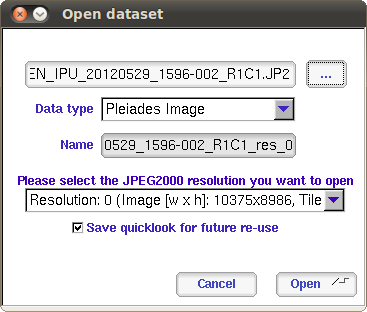
\includegraphics[width=0.4\textwidth]{../Art/MonteverdiImages/pleiades_open.png}
  \itkcaption[\mont \phr image opening]{Dialog window when opening a \phr image in \mont}
  \label{fig:pleiades_open}
\end{figure}

\begin{figure}
  \center
  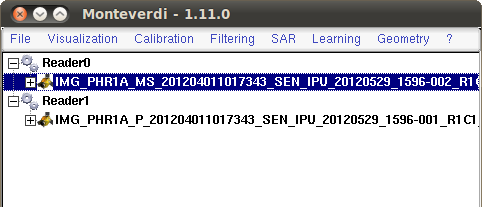
\includegraphics[width=0.5\textwidth]{../Art/MonteverdiImages/pleiades_monteverdi.png}
  \itkcaption[\phr dataset in \mont ]{\phr images in the main \mont window}
  \label{fig:pleiades_monteverdi}
\end{figure}

Figure~\ref{fig:pleiades_open}, page~\pageref{fig:pleiades_open} shows
the dialog box when opening a \phr image in \mont. One can see some
changes with respect to the classical dialog box for images opening.

The first novelty is a combo box allowing to choose the resolution of
the \jpg file one wants to decode. As said in the introduction of
this section, \otb can take advantage of \jpg capability to access
coarser resolution ver efficiently. If you select for instance
the \textit{Resolution: 1} item, you will end with an image half the
size of the original image with pixels twice as big. For instance, on
a \phr panchromatic or pansharpened product,
the \textit{Resolution: 0} image has a ground samping distance of
0.5 meters while the \textit{Resolution: 1} image has a ground
samping distance of one meter. For a multispectral product,
the \textit{Resolution: 0} image has a ground samping distance of 2
meters while the \textit{Resolution: 1} image has a ground samping
distance of 4 meters.

The second novelty is a check-box called \textit{Save quicklook for
future re-use}. This option allows to speed-up the loading of a
\phr image within \mont. In fact, when loading a \phr
image, \mont generates a quicklook of this image to be used as a
minimap in the \textit{Viewer Module} as well as in
the \textit{Uncompress Jpeg2000 image} module. This quicklook is the
coarser level of resolution from the \jpg file: it should decode
easily, but can still take a while. This is why if the check-box is
checked, \mont will write this quicklook in uncompressed \textit{Tiff}
format next to the \jpg file. For instance, if the file name  is:
\begin{scriptsize}
\begin{verbatim}
IMG_PHR1A_MS_201204011017343_SEN_IPU_20120529_1596-002_R1C1.JP2
\end{verbatim}
\end{scriptsize}

\mont will write, if it can, the following files in the same
directory:
\begin{scriptsize}
\begin{verbatim}
IMG_PHR1A_MS_201204011017343_SEN_IPU_20120529_1596-002_R1C1.JP2_ql_by_otb.tif
IMG_PHR1A_MS_201204011017343_SEN_IPU_20120529_1596-002_R1C1.JP2_ql_by_otb.geom
\end{verbatim}
\end{scriptsize}

Next time one will try to open this image in \mont, the application
will find these files and load directly the quicklook from them,
instead of decoding it from the \jpg file, resulting in an instant
loading of the image in \mont. Since the wheight of these extra files
is ususally of a few megaoctets, it is recommended to keep this option
checked unless one has a very good reason not to. Now that the \phr
image is loaded in \mont, it appears in the main \mont window, as
shown in figure~\ref{fig:pleiades_monteverdi},
page~\pageref{fig:pleiades_monteverdi}.


\subsection{Viewing a \phr image in \mont}

 You can open the \phr image in the viewer, either by using the
contextual menu or by opening the \textit{Viewer Module} through the
menu bar.

You can notice that the viewer opens quickly without showing the
traditional progress bar. This is because \mont already loaded the
quick-look upon opening, and we do not need to re-compute it each time
the image is opened in the \textit{Viewer Module}. 

\begin{figure}[!t]
  \center
  \includegraphics[width=0.9\textwidth]{../Art/MonteverdiImages/pleiades_viewer.png}
  \itkcaption[\phr image in \mont viewer]{A \phr image displayed
  in \mont viewer. \copyright CNES 2012}
  \label{fig:pleiades_viewer}
\end{figure}

Figure~\ref{fig:pleiades_viewer}, page~\pageref{fig:pleiades_viewer}
shows a \phr image displayed in the \textit{Viewer Module}. One can
notice that the navigation experience is rather smooth. If you
navigate using arrows keys, you will notice that latency can occur now
and then: this is due to the viewport switching to a new \jpg tile to
decode. On can also observe that the latitude and longitude of the
pixel under the mouse pointer is displayed, which means that the
sensor modelling is handled (if you have an internet connection, you
may even see the actual name of the place under mouse
pointer). Last, as said in the foreword of this section, \phr image
can be quite large, so it might be convenient to switch the viewer
style from \textit{Packed} to \textit{Splitted}, in which case you
will be able to maximize the \textit{Scroll Window} for better
localisation of the viewed area. To do so, one can go to
the \textit{Setup} tab of the \textit{Viewer Control Window}.

\subsection{Handling mega-tiles in \mont}

If the \phr product is very large, it might happen that the image is
actually splitted into several \jpg files, also called
mega-tiles. Since the area of interest might span two or more
mega-tiles, it is convenient to stitch together these tiles so as to
get the entire scene into one \mont dataset. To do so, one must first
open all mega-tiles in \mont, as described in
section~\ref{sec:mvd_phr_open}, page~\pageref{sec:mvd_phr_open}. Once
all mega-tiles are opened as shown in
figure~\ref{fig:pleiades_mtiles_open},
page~\pageref{fig:pleiades_mtiles_open}.

Once this is done, one can use the \textit{Mosaic Images module} from
the \textit{File} menu. Simply append all mega-tiles into the module
and run it: the module will look for the $RiCj$ pattern to determine
the mega-tiles layout, and will also check for consistency,
e.g. missing tiles or mega-tiles size mismatch. Upon success, it
generates a new \phr image dataset, which corresponding to the entire
scene, as shown in figure~\ref{fig:pleiades_mtiles_open},
page~\pageref{fig:pleiades_mtiles_open}. One can then use this dataset
as a regular \phr dataset.

\begin{figure}[!t]
  \center
  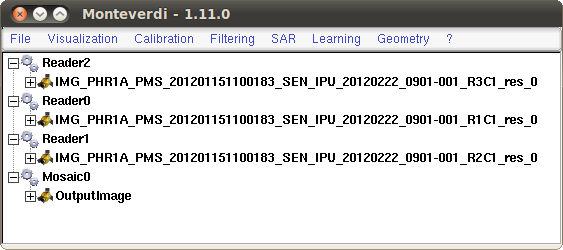
\includegraphics[width=0.4\textwidth]{../Art/MonteverdiImages/pleiades_mtiles_open.png}
  \itkcaption[Handling \phr mega-tiles in \mont]{\phr mega-tiles and
  output mosaic in \mont}
  \label{fig:pleiades_mtiles_open}
\end{figure}

\subsection{Partial uncompressing of \phr images in \mont}

The next very important thing one can do with \mont is to select an
area of interest in the \phr image so as to uncompress it to disk. To
do so, open the \phr dataset into the \textit{Uncompress Jpeg2000
image module} from the \textit{File}
menu. Figure~\ref{fig:pleiades_uncom},
page~\pageref{fig:pleiades_uncom} shows what this module looks
like. On the left, one can find informations about the images:
dimensions, resolution level, and number of \jpg tiles in image,
dimension of tiles, and size of tiles in mega-octets. The center part
of the module is the most important one: it displays a quick-look of
the \phr image. On this quick-look, one can select the area to be
decoded by drawing a rectangle with the mouse. The red rectangle shown
by the module corresponds to this user-defined area. On the left, in
red, one can find the start index and size of corresponding region.

The module also displays a green rectangle, which shows the minimum
set of tiles to be decoded to decode the red area: \textbf{this is the
region that will actually be decoded to disk}. On the left, in green,
one can find information about this region: how many tiles it
contains, and what will be the size of the corresponding decoded
output file.

Once one chose her area of interest, one can click on
the \textit{Save} button, and select an output file. The module will
write a geometry file (with the \textit{.geom} extension) with all
useful metadata in it, so that when reading back the file in \mont or
in \app, geometry and radiometry based functionalities can still be
used.

\begin{figure}[!t]
  \center
  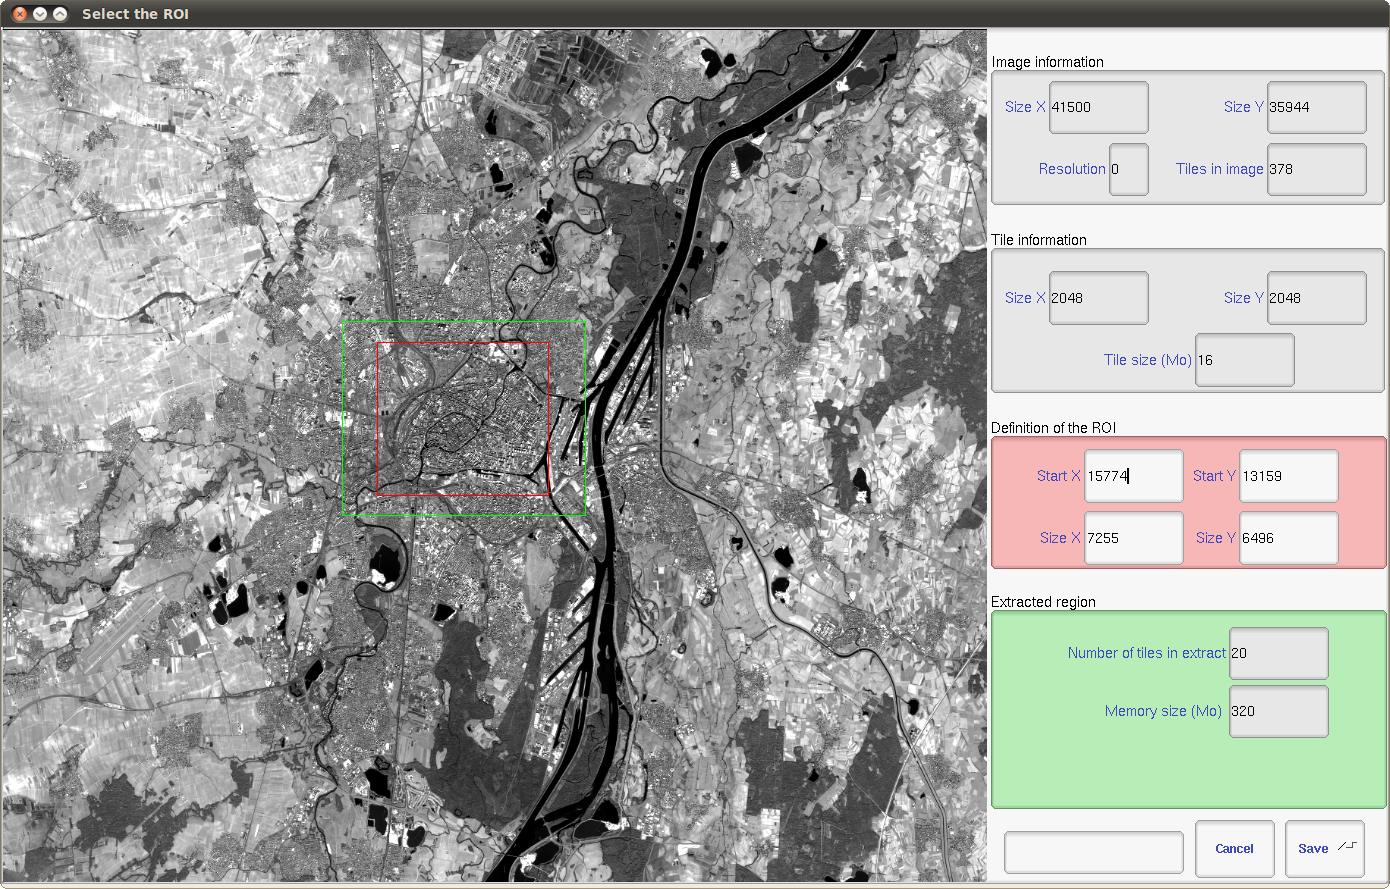
\includegraphics[width=0.9\textwidth]{../Art/MonteverdiImages/pleiades_uncom.png}
  \itkcaption[\mont \phr uncompress module]{A \phr image
  in \mont \textit{Uncompress Jpeg2000 image module.} \copyright CNES 2012}
  \label{fig:pleiades_uncom}
\end{figure}


\subsection{Other processing of \phr images with \mont}

For all the reasons exposed in the foreword of this section, we do not
allow to use directly \phr images in the remaining of \mont modules:
the advised way of doing so is to first uncompress the area of
interest to disk.

\subsection{Processing of \phr images with \app}

The \app are able to work directly with \phr images. However, keep in
mind that performances may be limited due to the reasons exposed in
the foreword of this section. If you experiment poor performances with
some application, try to uncompress the area of interest from your
image with \mont first. One can also use the \application{ExtractROI}
application for this purpose.

One thing that is interesting to know is that one can access the
coarser resolution of the \jpg file by appending $:i$ to the filename,
where $i$ is the resolution level starting at 0. For instance, one can
use the following:
\begin{scriptsize}
\begin{verbatim}
otbcli_ExtractROI -in IMG_PHR1A_PMS_201201151100183_SEN_IPU_20120222_0901-001_R2C1.JP2:5 -out test.tif uint16
\end{verbatim}
\end{scriptsize}
